\documentclass[pdftex,10pt,a4paper]{article}
\usepackage[utf8]{inputenc}
\usepackage[german]{babel}
\usepackage{wrapfig}
\usepackage{listings}
\usepackage{amsfonts}
\usepackage{fontenc}
\usepackage{amssymb}
\usepackage{graphicx}
\graphicspath{ {/home/slaan/git/bs3/doc/images/} }
\begin{document}


\title{BS Praktikum 3}
\author{Alex Mantel, Daniel Hofmeister}
\date{\today}
\maketitle
\newpage

\tableofcontents
\newpage

\section{Visualisierung der Strukturen und Parameter}
        
vmem\_struct
  vmem\_adm\_struct
  pt\_struct
    pt\_enty

\section{Vereinfachung der Bitmap}
Anstatt der Bitmap l\"asst sich eine Variable verwenden. Diese wird bei der Allokation der ersten 16 Pages verwendet, um bei jeder einzelnen Allokation eine die Page in eine Frame an der Stelle der Variable zu laden. Anschlie{\ss}end wird die Variable inkrementiert. Wenn die Variable bzw. der Z\"ahler den Wert 15 erreicht, soll f\"ur weitere Allokationen ein Ersetzungsverfahren verwendet werden.

\section{Skizze des Kommunikationsrahmen}
%\begin{figure}[h]
%  \caption{Kommunikationsrahmen}
%  \label{fig:kr}
%  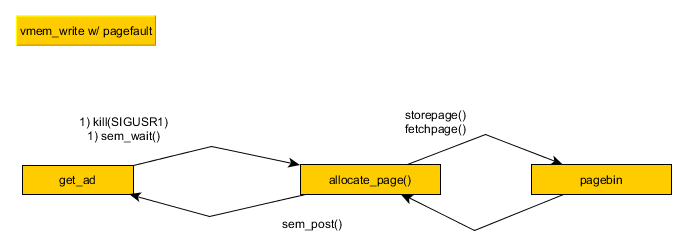
\includegraphics[scale=0.5]{communicationframe}
%\end{figure}

\section{Wie entscheiden wir die geforderte Seite}
\"Uber den flag "DVEM_ALGO" l\"asst sich bestimmen, mit welcher Strategie die pageersetzung erfolgen soll. Dabei gelten folgende Werte: 0=FIFO, 1=LRU, 2=CLOCK

\section{Wie finden die Zugriffe auf die Pagefile mit fwrite und fread statt?}
Die Befehl fwrite und fread nehmen 4 Parameter:
0) Anfangsadresse (Beginn der Page)
1) Gr\"osse in Bytes
2) Anzahl der Elemente 
3) Pfadname der Zieldatei

Man braucht nur eine Page in den Hauptspeicher zu schreiben (in unserem Fall in die pagefile.bin) wenn das DirtyBit gesetzt ist, also diese Datei verändert wurde.

\section{Aufrufreihenfolge der Funktionen in mmanage.h}
mmanager wird zuerst initialisiert über die main-methode. In dieser werden folgende Methoden aufgerufen:
init_pagefile
vmem_init
sighandler wird initalisiert

Anschließend werden über den signal handler die anderen Methoden erreicht. Die Signale bewirken folgende Prozeduren:
SIGUSR1:
allocate_page (sucht eine die aus adm.req_pageno geforderte page)
	search_bitmap  (suche nach noch nicht verwendetem frame)
		find_free_bit
	find_remove_frame (entscheider für strategie für pageersetzung, da hier page aus pagefile.bin geladen werden muss)
		find_remove_fifo OR
		find_remove_lru OR
		find_remove_clock OR
	store_page (speicherung der zu ersetzenden page wenn dirtybit gesetzt)
	update_pt (pagetable aktualisieren)
	fetch_page (gesuchte page laden)
	logger	(logging information in datei schreiben)
	
SIGUSR2:
dump_pt (inhalt der pagetable ausgeben)

SITINT:
cleanup (schließen der files, freigabe des shared memory)

\section{Sukzessive Sequenzdiagramm}


\section{Welche Funktionen setzen die Flags Present, Dirty und Used?}
Present: mmanage:update_pt
Used: mmanage:update_pt
Dirty: vmaccess: get_ad

\bibliographystyle{alpha}
\bibliography{./references}
\end{document}
